
\documentclass{tufte-book}

%%% Disable auxiliary files
% These are used for references in latex documents, which are handled by
% disseminate. Additionally, aux files can trip up compiles of PDFs.
\nofiles

%%%
% Graphics
\usepackage{graphicx}

%%%
% Caption customization
\usepackage[labelformat=empty]{caption}

%%%
% title, section labels
\usepackage{titlesec}

%%%
% Panels for figures
\newenvironment{panel}[1]
{\begin{minipage}{ #1}\footnotesize}
{\end{minipage}}

%%%
% Load UTF-8 characters
% \usepackage[T1]{fontenc}  % introduces grainy bitmap fonts
\usepackage[utf8]{inputenc}
\DeclareUnicodeCharacter{26AC}{\circ}  % used for degrees
\DeclareUnicodeCharacter{25CB}{\ensuremath{\circ}}  % used for degrees
\DeclareUnicodeCharacter{00A7}{^^a7}

%%%
% Lists
\usepackage{easylist}

\usepackage{enumitem}
\setlistdepth{9}

%%%
% Math
\usepackage[fleqn]{amsmath}
\usepackage{mathtools}
\usepackage{bm}

%%%
% Hyperref package for links
\usepackage{hyperref}
\hypersetup{ %colorlinks,
            %linkcolor=black!50!blue,
            %filecolor=black!50!blue,pdftitle=Fundamentals of NMR Spectroscopy,pdfauthor=Justin Lorieau,
            pdfcreator=Disseminate
            }

%%%
% Page Layout
\usepackage{geometry}
% Increase text height and bottom margin
\geometry{
  textheight=48\baselineskip,
  textwidth=114mm, % main text block
  marginparsep=8mm, % gutter between main text block and margin notes
  marginparwidth=55mm, % width of margin notes
}
\setlength{\evensidemargin}{-0.5in}

%%%
% Colors
\usepackage{xcolor}

%%%
% Counters
\newcounter{title}

%%% 
% Symbols
\renewcommand{\deg}{^\circ}

%%%
% Nice tables
\usepackage{booktabs}

%%%
% Color boxes
\usepackage[breakable]{tcolorbox}

\newtcolorbox{featurebox}{colback=black!5!white,
                          colframe=black!40!white,
                          breakable,
                          before skip=\baselineskip,
                          after skip=\baselineskip}
\newtcolorbox{examplebox}{colback=blue!5!white,
                          colframe=blue!40!white,
                          breakable,
                          before skip=\baselineskip,
                          after skip=\baselineskip}
\newtcolorbox{problembox}{colback=green!7!white,
                          colframe=green!50!black!40!white,
                          breakable,
                          before skip=\baselineskip,
                          after skip=\baselineskip}
\usepackage{fancyvrb}

\makeatletter
\def\PY@reset{\let\PY@it=\relax \let\PY@bf=\relax%
    \let\PY@ul=\relax \let\PY@tc=\relax%
    \let\PY@bc=\relax \let\PY@ff=\relax}
\def\PY@tok#1{\csname PY@tok@#1\endcsname}
\def\PY@toks#1+{\ifx\relax#1\empty\else%
    \PY@tok{#1}\expandafter\PY@toks\fi}
\def\PY@do#1{\PY@bc{\PY@tc{\PY@ul{%
    \PY@it{\PY@bf{\PY@ff{#1}}}}}}}
\def\PY#1#2{\PY@reset\PY@toks#1+\relax+\PY@do{#2}}

\expandafter\def\csname PY@tok@w\endcsname{\def\PY@tc##1{\textcolor[rgb]{0.73,0.73,0.73}{##1}}}
\expandafter\def\csname PY@tok@c\endcsname{\let\PY@it=\textit\def\PY@tc##1{\textcolor[rgb]{0.25,0.50,0.50}{##1}}}
\expandafter\def\csname PY@tok@cp\endcsname{\def\PY@tc##1{\textcolor[rgb]{0.74,0.48,0.00}{##1}}}
\expandafter\def\csname PY@tok@k\endcsname{\let\PY@bf=\textbf\def\PY@tc##1{\textcolor[rgb]{0.00,0.50,0.00}{##1}}}
\expandafter\def\csname PY@tok@kp\endcsname{\def\PY@tc##1{\textcolor[rgb]{0.00,0.50,0.00}{##1}}}
\expandafter\def\csname PY@tok@kt\endcsname{\def\PY@tc##1{\textcolor[rgb]{0.69,0.00,0.25}{##1}}}
\expandafter\def\csname PY@tok@o\endcsname{\def\PY@tc##1{\textcolor[rgb]{0.40,0.40,0.40}{##1}}}
\expandafter\def\csname PY@tok@ow\endcsname{\let\PY@bf=\textbf\def\PY@tc##1{\textcolor[rgb]{0.67,0.13,1.00}{##1}}}
\expandafter\def\csname PY@tok@nb\endcsname{\def\PY@tc##1{\textcolor[rgb]{0.00,0.50,0.00}{##1}}}
\expandafter\def\csname PY@tok@nf\endcsname{\def\PY@tc##1{\textcolor[rgb]{0.00,0.00,1.00}{##1}}}
\expandafter\def\csname PY@tok@nc\endcsname{\let\PY@bf=\textbf\def\PY@tc##1{\textcolor[rgb]{0.00,0.00,1.00}{##1}}}
\expandafter\def\csname PY@tok@nn\endcsname{\let\PY@bf=\textbf\def\PY@tc##1{\textcolor[rgb]{0.00,0.00,1.00}{##1}}}
\expandafter\def\csname PY@tok@ne\endcsname{\let\PY@bf=\textbf\def\PY@tc##1{\textcolor[rgb]{0.82,0.25,0.23}{##1}}}
\expandafter\def\csname PY@tok@nv\endcsname{\def\PY@tc##1{\textcolor[rgb]{0.10,0.09,0.49}{##1}}}
\expandafter\def\csname PY@tok@no\endcsname{\def\PY@tc##1{\textcolor[rgb]{0.53,0.00,0.00}{##1}}}
\expandafter\def\csname PY@tok@nl\endcsname{\def\PY@tc##1{\textcolor[rgb]{0.63,0.63,0.00}{##1}}}
\expandafter\def\csname PY@tok@ni\endcsname{\let\PY@bf=\textbf\def\PY@tc##1{\textcolor[rgb]{0.60,0.60,0.60}{##1}}}
\expandafter\def\csname PY@tok@na\endcsname{\def\PY@tc##1{\textcolor[rgb]{0.49,0.56,0.16}{##1}}}
\expandafter\def\csname PY@tok@nt\endcsname{\let\PY@bf=\textbf\def\PY@tc##1{\textcolor[rgb]{0.00,0.50,0.00}{##1}}}
\expandafter\def\csname PY@tok@nd\endcsname{\def\PY@tc##1{\textcolor[rgb]{0.67,0.13,1.00}{##1}}}
\expandafter\def\csname PY@tok@s\endcsname{\def\PY@tc##1{\textcolor[rgb]{0.73,0.13,0.13}{##1}}}
\expandafter\def\csname PY@tok@sd\endcsname{\let\PY@it=\textit\def\PY@tc##1{\textcolor[rgb]{0.73,0.13,0.13}{##1}}}
\expandafter\def\csname PY@tok@si\endcsname{\let\PY@bf=\textbf\def\PY@tc##1{\textcolor[rgb]{0.73,0.40,0.53}{##1}}}
\expandafter\def\csname PY@tok@se\endcsname{\let\PY@bf=\textbf\def\PY@tc##1{\textcolor[rgb]{0.73,0.40,0.13}{##1}}}
\expandafter\def\csname PY@tok@sr\endcsname{\def\PY@tc##1{\textcolor[rgb]{0.73,0.40,0.53}{##1}}}
\expandafter\def\csname PY@tok@ss\endcsname{\def\PY@tc##1{\textcolor[rgb]{0.10,0.09,0.49}{##1}}}
\expandafter\def\csname PY@tok@sx\endcsname{\def\PY@tc##1{\textcolor[rgb]{0.00,0.50,0.00}{##1}}}
\expandafter\def\csname PY@tok@m\endcsname{\def\PY@tc##1{\textcolor[rgb]{0.40,0.40,0.40}{##1}}}
\expandafter\def\csname PY@tok@gh\endcsname{\let\PY@bf=\textbf\def\PY@tc##1{\textcolor[rgb]{0.00,0.00,0.50}{##1}}}
\expandafter\def\csname PY@tok@gu\endcsname{\let\PY@bf=\textbf\def\PY@tc##1{\textcolor[rgb]{0.50,0.00,0.50}{##1}}}
\expandafter\def\csname PY@tok@gd\endcsname{\def\PY@tc##1{\textcolor[rgb]{0.63,0.00,0.00}{##1}}}
\expandafter\def\csname PY@tok@gi\endcsname{\def\PY@tc##1{\textcolor[rgb]{0.00,0.63,0.00}{##1}}}
\expandafter\def\csname PY@tok@gr\endcsname{\def\PY@tc##1{\textcolor[rgb]{1.00,0.00,0.00}{##1}}}
\expandafter\def\csname PY@tok@ge\endcsname{\let\PY@it=\textit}
\expandafter\def\csname PY@tok@gs\endcsname{\let\PY@bf=\textbf}
\expandafter\def\csname PY@tok@gp\endcsname{\let\PY@bf=\textbf\def\PY@tc##1{\textcolor[rgb]{0.00,0.00,0.50}{##1}}}
\expandafter\def\csname PY@tok@go\endcsname{\def\PY@tc##1{\textcolor[rgb]{0.53,0.53,0.53}{##1}}}
\expandafter\def\csname PY@tok@gt\endcsname{\def\PY@tc##1{\textcolor[rgb]{0.00,0.27,0.87}{##1}}}
\expandafter\def\csname PY@tok@err\endcsname{\def\PY@bc##1{\setlength{\fboxsep}{0pt}\fcolorbox[rgb]{1.00,0.00,0.00}{1,1,1}{\strut ##1}}}
\expandafter\def\csname PY@tok@kc\endcsname{\let\PY@bf=\textbf\def\PY@tc##1{\textcolor[rgb]{0.00,0.50,0.00}{##1}}}
\expandafter\def\csname PY@tok@kd\endcsname{\let\PY@bf=\textbf\def\PY@tc##1{\textcolor[rgb]{0.00,0.50,0.00}{##1}}}
\expandafter\def\csname PY@tok@kn\endcsname{\let\PY@bf=\textbf\def\PY@tc##1{\textcolor[rgb]{0.00,0.50,0.00}{##1}}}
\expandafter\def\csname PY@tok@kr\endcsname{\let\PY@bf=\textbf\def\PY@tc##1{\textcolor[rgb]{0.00,0.50,0.00}{##1}}}
\expandafter\def\csname PY@tok@bp\endcsname{\def\PY@tc##1{\textcolor[rgb]{0.00,0.50,0.00}{##1}}}
\expandafter\def\csname PY@tok@fm\endcsname{\def\PY@tc##1{\textcolor[rgb]{0.00,0.00,1.00}{##1}}}
\expandafter\def\csname PY@tok@vc\endcsname{\def\PY@tc##1{\textcolor[rgb]{0.10,0.09,0.49}{##1}}}
\expandafter\def\csname PY@tok@vg\endcsname{\def\PY@tc##1{\textcolor[rgb]{0.10,0.09,0.49}{##1}}}
\expandafter\def\csname PY@tok@vi\endcsname{\def\PY@tc##1{\textcolor[rgb]{0.10,0.09,0.49}{##1}}}
\expandafter\def\csname PY@tok@vm\endcsname{\def\PY@tc##1{\textcolor[rgb]{0.10,0.09,0.49}{##1}}}
\expandafter\def\csname PY@tok@sa\endcsname{\def\PY@tc##1{\textcolor[rgb]{0.73,0.13,0.13}{##1}}}
\expandafter\def\csname PY@tok@sb\endcsname{\def\PY@tc##1{\textcolor[rgb]{0.73,0.13,0.13}{##1}}}
\expandafter\def\csname PY@tok@sc\endcsname{\def\PY@tc##1{\textcolor[rgb]{0.73,0.13,0.13}{##1}}}
\expandafter\def\csname PY@tok@dl\endcsname{\def\PY@tc##1{\textcolor[rgb]{0.73,0.13,0.13}{##1}}}
\expandafter\def\csname PY@tok@s2\endcsname{\def\PY@tc##1{\textcolor[rgb]{0.73,0.13,0.13}{##1}}}
\expandafter\def\csname PY@tok@sh\endcsname{\def\PY@tc##1{\textcolor[rgb]{0.73,0.13,0.13}{##1}}}
\expandafter\def\csname PY@tok@s1\endcsname{\def\PY@tc##1{\textcolor[rgb]{0.73,0.13,0.13}{##1}}}
\expandafter\def\csname PY@tok@mb\endcsname{\def\PY@tc##1{\textcolor[rgb]{0.40,0.40,0.40}{##1}}}
\expandafter\def\csname PY@tok@mf\endcsname{\def\PY@tc##1{\textcolor[rgb]{0.40,0.40,0.40}{##1}}}
\expandafter\def\csname PY@tok@mh\endcsname{\def\PY@tc##1{\textcolor[rgb]{0.40,0.40,0.40}{##1}}}
\expandafter\def\csname PY@tok@mi\endcsname{\def\PY@tc##1{\textcolor[rgb]{0.40,0.40,0.40}{##1}}}
\expandafter\def\csname PY@tok@il\endcsname{\def\PY@tc##1{\textcolor[rgb]{0.40,0.40,0.40}{##1}}}
\expandafter\def\csname PY@tok@mo\endcsname{\def\PY@tc##1{\textcolor[rgb]{0.40,0.40,0.40}{##1}}}
\expandafter\def\csname PY@tok@ch\endcsname{\let\PY@it=\textit\def\PY@tc##1{\textcolor[rgb]{0.25,0.50,0.50}{##1}}}
\expandafter\def\csname PY@tok@cm\endcsname{\let\PY@it=\textit\def\PY@tc##1{\textcolor[rgb]{0.25,0.50,0.50}{##1}}}
\expandafter\def\csname PY@tok@cpf\endcsname{\let\PY@it=\textit\def\PY@tc##1{\textcolor[rgb]{0.25,0.50,0.50}{##1}}}
\expandafter\def\csname PY@tok@c1\endcsname{\let\PY@it=\textit\def\PY@tc##1{\textcolor[rgb]{0.25,0.50,0.50}{##1}}}
\expandafter\def\csname PY@tok@cs\endcsname{\let\PY@it=\textit\def\PY@tc##1{\textcolor[rgb]{0.25,0.50,0.50}{##1}}}

\def\PYZbs{\char`\\}
\def\PYZus{\char`\_}
\def\PYZob{\char`\{}
\def\PYZcb{\char`\}}
\def\PYZca{\char`\^}
\def\PYZam{\char`\&}
\def\PYZlt{\char`\<}
\def\PYZgt{\char`\>}
\def\PYZsh{\char`\#}
\def\PYZpc{\char`\%}
\def\PYZdl{\char`\$}
\def\PYZhy{\char`\-}
\def\PYZsq{\char`\'}
\def\PYZdq{\char`\"}
\def\PYZti{\char`\~}
% for compatibility with earlier versions
\def\PYZat{@}
\def\PYZlb{[}
\def\PYZrb{]}
\makeatother
%%%
% Remove labels from captions  
\usepackage{etoolbox}
\makeatletter
\patchcmd{\@caption}
  {\noindent\csname fnum@#1\endcsname: \ignorespaces}
  {\noindent}
  {}{}
\makeatother

%%%
% Format chapter headings
\usepackage[Bjornstrup]{fncychap}
\setcounter{secnumdepth}{0} % turn on numbering for parts and chapters
\title{
        Fundamentals of NMR Spectroscopy
    }
    \author{
        Justin Lorieau
    }

\begin{document}
\mainmatter  % Needed to set chapter/section numbering
\setcounter{chapter}{1}
\chapter{Refocused INEPT, Delayed Decoupling and In-Phase Spectra} \label{ch:fundamental-solnnmr-inept-ref-inept-dm-refocused-inept-delayed-decoupling-and-in-phase-spectra}

Justin Lorieau

The refocused INEPT sequence\marginnote{Burum D., Ernst R. Net polarization
  transfer via a J-ordered state for signal enhancement of low-sensitivity
  nuclei. J Magn Reson. 1980 Apr;39(1):163–168. }
(\href{#fig:ref-inept_ref-inept}{Fig. 2.1}) converts the anti-phase
magnetization of the INEPT sequence into in-phase magnetization, while
still benefiting from the signal enhancement of the INEPT
sequence. This approach has the advantage that the spectrum can be
decoupled to produce singlet peaks.
\setcounter{section}{0}
\section{2.1. Theory} \label{sec:fundamental-solnnmr-inept-ref-inept-dm-theory}
\begin{marginfigure}
  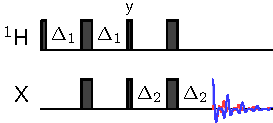
\includegraphics{{tex/media/ref-inept_3533f613ccb5}.pdf}
    \caption{\textbf{Fig. 2.1}. The refocused INEPT experiment.} \label{fig:ref-inept_ref-inept}
  
\end{marginfigure}

\begin{marginfigure}
  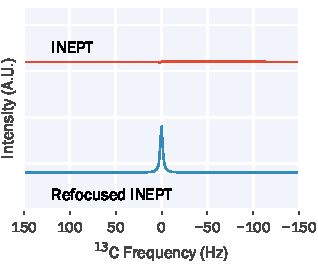
\includegraphics{{tex/media/plots/ref-inept/inept_vs_ref_inept_H-dcpl}.pdf}
  \caption{\textbf{Fig. 2.2}. Comparison of \ensuremath{^{13}}C spectra for the INEPT sequence and
    refocused INEPT sequence with \ensuremath{^{1}}H decoupling during
    \ensuremath{^{13}}C acquisition.} \label{fig:inept_inept_v_refinept_H-dcpl}
\end{marginfigure}

The INEPT sequence produces
anti-phase magnetization (\textit{e.g.} \ensuremath{\boldsymbol{-2H_zC_y}}) with peaks of
opposite sign, and the refocused INEPT produces in-phase
magnetization (\textit{e.g.} \ensuremath{\boldsymbol{C_z}}) with peaks of the same
sign. When \ensuremath{^{1}}H decoupling is applied to the anti-phase
magnetization of the INEPT sequence, the peaks cancel each other
to produce a null spectrum. The objective of the refocused INEPT
and DEPT experiments is to produce in-phase magnetization that can be
decoupled to produce singlet peaks.
\setcounter{subsection}{0}
\subsection{2.1.1. Methine, Amide and the AX Spin System} \label{subsec:fundamental-solnnmr-inept-ref-inept-dm-methine-amide-and-the-ax-spin-system}
The \textit{refocused} INEPT sequence produces in-phase magnetization
that can \ensuremath{^{1}}H decoupled to produce high intensity singlet peaks.

In this example, we’ll use a \ensuremath{^{1}}H spin bonded to a \ensuremath{^{13}}C
spin. If we use a delay, \ensuremath{\Delta_1 = (4 J_{CH})^{-1}}, the first step
of the sequence is simply an INEPT sequence (\href{#fig:ref-inept_ref-inept_step1}{Fig. 2.3}).
\begin{alignat*}{3} %
\boldsymbol{H_z} & \xrightarrow{\mathmakebox[4em]{\text{INEPT}}} && \boldsymbol{-2 H_z C_y}
\end{alignat*}
\begin{marginfigure}
  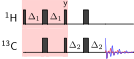
\includegraphics{{tex/media/ref-inept_bff6eb2a6dad}.pdf}
  \caption{\textbf{Fig. 2.3}. The first step of the refocused INEPT sequence highlighted in
  red.} \label{fig:ref-inept_ref-inept_step1}
\end{marginfigure}

In the second step, we’ll only propagate the J\ensuremath{_{CH}}-coupling since the
`\ensuremath{\Delta_2-180^{○}_{x} (^{13}C)-\Delta_2}' pulse sequence block
refocuses the \ensuremath{^{13}}C chemical shifts (\href{#fig:ref-inept_ref-inept_step2}{Fig. 2.4}).
Thereafter, we’ll apply the two 180\ensuremath{^{○}} pulses.
\begin{align*} %
\xrightarrow{\mathmakebox[7em]{\Delta_2}} &
    \boldsymbol{-2 H_z C_y} \cos (\pi J_{CH} \Delta_2) +
    \boldsymbol{C_x} \sin (\pi J_{CH} \Delta_2) \displaybreak[2] \\[0.5em]
  \xrightarrow{\mathmakebox[7em]{180^{○}_{x} (^{1}H),\ 180^{○}_{x} (^{13}C)}}
  &
  \boldsymbol{-2 H_z C_y} \cos (\pi J_{CH} \Delta_2) +
  \boldsymbol{C_x} \sin (\pi J_{CH} \Delta_2)
\end{align*}
\begin{marginfigure}
    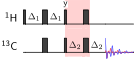
\includegraphics{{tex/media/ref-inept_9781760da605}.pdf}
  \caption{\textbf{Fig. 2.4}. The second step of the refocused INEPT sequence highlighted
   in red.} \label{fig:ref-inept_ref-inept_step2}
\end{marginfigure}

The final and third step (\href{#fig:ref-inept_ref-inept_step3}{Fig. 2.5}) propagates
the magnetization with another \ensuremath{\Delta_2} period.
\begin{align*} %
\xrightarrow{\mathmakebox[7em]{\Delta_2}}&
  - \boldsymbol{2 H_z C_y} \cos (\pi J_{CH} \Delta_2) \cos(\pi J_{CH} \Delta_2) \\
  &
  + \boldsymbol{C_x} \cos (\pi J_{CH} \Delta_2) \sin(\pi J_{CH} \Delta_2) \\
  &
  + \boldsymbol{C_x} \sin (\pi J_{CH} \Delta_2) \cos (\pi J_{CH} \Delta_2) \\
  &
  + \boldsymbol{2 H_z C_y} \sin (\pi J_{CH} \Delta_2) \sin (\pi J_{CH} \Delta_2) \displaybreak[2] \\[0.5em]
  =&
  - \boldsymbol{2 H_z C_y} \cos(\pi J_{CH} 2 \Delta_2) + \boldsymbol{C_x} \sin(2 \pi J_{CH} \Delta_2)
\end{align*}
\begin{marginfigure}
  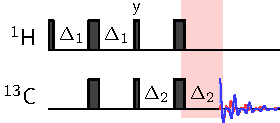
\includegraphics{{tex/media/ref-inept_47588112ea3f}.pdf}
  \caption{\textbf{Fig. 2.5}. The third step of the refocused INEPT sequence highlighted in red.} \label{fig:ref-inept_ref-inept_step3}
\end{marginfigure}

The \ensuremath{\boldsymbol{C_x}} term is maximum when \ensuremath{\Delta_2 = (4 J_{CH})^{-1}}. As with
the INEPT sequence, the \ensuremath{\boldsymbol{C_x}} magnetization is enhanced by a
factor \ensuremath{\frac{K_H}{K_C}} over the unenhanced version.

For a \ensuremath{^{13}}C-INEPT between for a \ensuremath{^{1}}H spin bonded to
a \ensuremath{^{13}}C (J\ensuremath{_{CH}} = 145 Hz), the magnetization after the
 is \ensuremath{\boldsymbol{2 H_z C_y}}. The refocused INEPT experiment
produces in-phase magnetization, \ensuremath{\boldsymbol{C_x}}, suitable for \ensuremath{^{1}}H
decoupling (\href{#fig:inept_inept_v_refinept}{Fig. 2.6}).

\begin{figure}
  \begin{panel}{0.32\textwidth}
    a. Magnetization after INEPT
    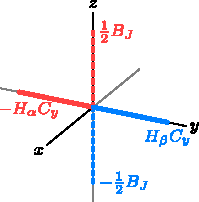
\includegraphics[width=0.99\textwidth]{{tex/media/asy/ref-inept/CH_before}.pdf}
  
\end{panel}
  \begin{panel}{0.32\textwidth}
    b. Magnetization after ref-INEPT
    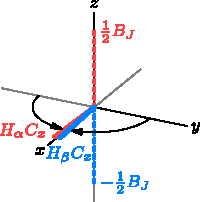
\includegraphics[width=0.99\textwidth]{{tex/media/asy/ref-inept/CH_after}.pdf}
  
\end{panel}
  \begin{panel}{0.32\textwidth}
    c. Comparison of Spectra
    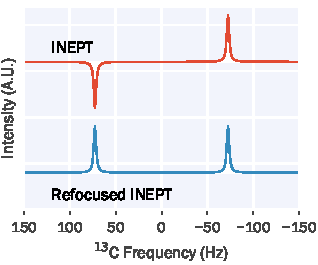
\includegraphics[width=0.99\textwidth]{{tex/media/plots/ref-inept/inept_vs_ref_inept}.pdf}
  
\end{panel}
  \caption{\textbf{Fig. 2.6}. Comparison of the INEPT sequence and the refocused
    INEPT sequence for a CH group.} \label{fig:inept_inept_v_refinept}
\end{figure}
\setcounter{subsection}{1}
\subsection{2.1.2. Cosine and Sine Modulation} \label{subsec:fundamental-solnnmr-inept-ref-inept-dm-cosine-and-sine-modulation}\setcounter{subsection}{2}
\subsection{2.1.3. Methylene, Methyl, AX2 and AX3 Spin Systems} \label{subsec:fundamental-solnnmr-inept-ref-inept-dm-methylene-methyl-ax2-and-ax3-spin-systems}
Different \ensuremath{\Delta_2} periods emphasize different types of spin
systems. Varying \ensuremath{\Delta_2} periods is commonly used to differentiate
between CH, CH\ensuremath{_{2}} and CH\ensuremath{_{3}} groups. This principal applies to
other X spins, such as \ensuremath{^{15}}N, but in the case of
NH\ensuremath{_{2}} and NH\ensuremath{_{3}} groups, rapid hydrogen
exchange with the solvent may impede the discrimination between these groups.

The initial INEPT period behaves the same for CH, CH\ensuremath{_{2}} and
CH\ensuremath{_{3}} groups. This is because each \ensuremath{^{1}}H spin is only bonded to
one \ensuremath{^{13}}C spin.

Once the magnetization is converted to transverse magnetization for
the \ensuremath{^{13}}C spin, the magnetization evolves with J-couplings to
multiple \ensuremath{^{1}}H spins during the rest of the refocused INEPT. This
is because, from the \ensuremath{^{13}}C spin’s perspective, a CH group
appears as a doublet, a CH\ensuremath{_{2}} group appears as a triplet and a CH\ensuremath{_{3}}
group appears as a quartet.

The conversion to \ensuremath{\boldsymbol{C_x}} magnetization follows different time
dependencies for the CH (AX), CH\ensuremath{_{2}} (AX2) and CH\ensuremath{_{3}} (AX3) groups.


\end{document}
